% $Id: template.tex 11 2007-04-03 22:25:53Z jpeltier $

\documentclass{vgtc}                          % final (conference style)
%\documentclass[review]{vgtc}                 % review
%\documentclass[widereview]{vgtc}             % wide-spaced review
%\documentclass[preprint]{vgtc}               % preprint
%\documentclass[electronic]{vgtc}             % electronic version

%% Uncomment one of the lines above depending on where your paper is
%% in the conference process. ``review'' and ``widereview'' are for review
%% submission, ``preprint'' is for pre-publication, and the final version
%% doesn't use a specific qualifier. Further, ``electronic'' includes
%% hyperreferences for more convenient online viewing.

%% Please use one of the ``review'' options in combination with the
%% assigned online id (see below) ONLY if your paper uses a double blind
%% review process. Some conferences, like IEEE Vis and InfoVis, have NOT
%% in the past.

%% Figures should be in CMYK or Grey scale format, otherwise, colour
%% shifting may occur during the printing process.

%% These few lines make a distinction between latex and pdflatex calls and they
%% bring in essential packages for graphics and font handling.
%% Note that due to the \DeclareGraphicsExtensions{} call it is no longer necessary
%% to provide the the path and extension of a graphics file:
%% \includegraphics{diamondrule} is completely sufficient.
%%
\ifpdf%                                % if we use pdflatex
  \pdfoutput=1\relax                   % create PDFs from pdfLaTeX
  \pdfcompresslevel=9                  % PDF Compression
  \pdfoptionpdfminorversion=7          % create PDF 1.7
  \ExecuteOptions{pdftex}
  \usepackage{graphicx}                % allow us to embed graphics files
  \DeclareGraphicsExtensions{.pdf,.png,.jpg,.jpeg} % for pdflatex we expect .pdf, .png, or .jpg files
\else%                                 % else we use pure latex
  \ExecuteOptions{dvips}
  \usepackage{graphicx}                % allow us to embed graphics files
  \DeclareGraphicsExtensions{.eps}     % for pure latex we expect eps files
\fi%

%% it is recomended to use ``\autoref{sec:bla}'' instead of ``Fig.~\ref{sec:bla}''
\graphicspath{{figures/}{pictures/}{images/}{./}} % where to search for the images

\usepackage{microtype}                 % use micro-typography (slightly more compact, better to read)
\PassOptionsToPackage{warn}{textcomp}  % to address font issues with \textrightarrow
\usepackage{textcomp}                  % use better special symbols
\usepackage{mathptmx}                  % use matching math font
\usepackage{times}                     % we use Times as the main font
\renewcommand*\ttdefault{txtt}         % a nicer typewriter font
\usepackage{cite}                      % needed to automatically sort the references
\usepackage{tabu}                      % only used for the table example
\usepackage{booktabs}                  % only used for the table example
\usepackage{graphicx}
\usepackage{subfig}
%% We encourage the use of mathptmx for consistent usage of times font
%% throughout the proceedings. However, if you encounter conflicts
%% with other math-related packages, you may want to disable it.
\usepackage{color}
\newcommand{\todo}[1]{{\color{red}\bfseries [[#1]]}}

%% If you are submitting a paper to a conference for review with a double
%% blind reviewing process, please replace the value ``0'' below with your
%% OnlineID. Otherwise, you may safely leave it at ``0''.
\onlineid{0}

%% declare the category of your paper, only shown in review mode
\vgtccategory{Research}

%% allow for this line if you want the electronic option to work properly
\vgtcinsertpkg

%% In preprint mode you may define your own headline.
%\preprinttext{To appear in an IEEE VGTC sponsored conference.}

%% Paper title.

\title{HDI Visualization}

%% This is how authors are specified in the conference style

%% Author and Affiliation (single author).
%%\author{Roy G. Biv\thanks{e-mail: roy.g.biv@aol.com}}
%%\affiliation{\scriptsize Allied Widgets Research}

%% Author and Affiliation (multiple authors with single affiliations).
%%\author{Roy G. Biv\thanks{e-mail: roy.g.biv@aol.com} %
%%\and Ed Grimley\thanks{e-mail:ed.grimley@aol.com} %
%%\and Martha Stewart\thanks{e-mail:martha.stewart@marthastewart.com}}
%%\affiliation{\scriptsize Martha Stewart Enterprises \\ Microsoft Research}

%% Author and Affiliation (multiple authors with multiple affiliations)
\author{Xinyao Huang\thanks{e-mail: xhuang62@illinois.edu}\\ %
        \scriptsize University of Illinois at Urbana-Champaign %
\and Siwakorn Srisakaokul\thanks{e-mail: srisaka2@illinois.edu}\\ %
     \scriptsize University of Illinois at Urbana-Champaign}

%% A teaser figure can be included as follows, but is not recommended since
%% the space is now taken up by a full width abstract.
%\teaser{
%  \includegraphics[width=1.5in]{sample.eps}
%  \caption{Lookit! Lookit!}
%}

%% Abstract section.
\abstract{
Human Development Index (HDI) is used for assessing the development of a country, which can be useful for comparing national policy choices between two countries. In the past several decades, the HDI is calculated for each country to show how much the country has been developed. There are many HDI data available on the United Nations Development Programme (UNDP), which shows the values of the HDI and its components of each single country, but it does not represent other information such as the relationship between a country location and its HDI, and correlation between \textit{mean years of schooling} and \textit{expected year of schooling} (both are components in the HDI). In this project, we implement a tool that can visualize not only the HDI information for each country along with the country's location but also a parallel coordinate plot to show the relationship between the HDI and its components for all the countries. Moreover, we can see how much countries develop over the past several years. With the tool, we can observe interesting findings. For example, the countries located in the lower part of the earth tend to have low expected years of schooling.
} % end of abstract

%% ACM Computing Classification System (CCS).
%% See <http://www.acm.org/about/class> for details.
%% We recommend the 2012 system <http://www.acm.org/about/class/class/2012>
%% For the 2012 system use the ``\CCScatTwelve'' which command takes four arguments.
%% The 1998 system <http://www.acm.org/about/class/class/2012> is still possible
%% For the 1998 system use the ``\CCScat'' which command takes four arguments.
%% In both cases the last two arguments (1998) or last three (2012) can be empty.

\CCScatlist{
  \CCScatTwelve{Scientific visualization}{}{}{};
  \CCScatTwelve{Human Development Index}{}{}{};
  \CCScatTwelve{Country map}{}{}{};
  \CCScatTwelve{Parallel coordinates}{}{}{};
}

%\CCScatlist{
  %\CCScat{H.5.2}{User Interfaces}{User Interfaces}{Graphical user interfaces (GUI)}{};
  %\CCScat{H.5.m}{Information Interfaces and Presentation}{Miscellaneous}{}{}
%}

%% Copyright space is enabled by default as required by guidelines.
%% It is disabled by the 'review' option or via the following command:
% \nocopyrightspace

%%%%%%%%%%%%%%%%%%%%%%%%%%%%%%%%%%%%%%%%%%%%%%%%%%%%%%%%%%%%%%%%
%%%%%%%%%%%%%%%%%%%%%% START OF THE PAPER %%%%%%%%%%%%%%%%%%%%%%
%%%%%%%%%%%%%%%%%%%%%%%%%%%%%%%%%%%%%%%%%%%%%%%%%%%%%%%%%%%%%%%%%

\begin{document}
%% The ``\maketitle'' command must be the first command after the
%% ``\begin{document}'' command. It prepares and prints the title block.

%% the only exception to this rule is the \firstsection command
\firstsection{Introduction}

\maketitle
HDI is an useful index that shows how much a country has been developed over a year in term of human development. The HDI value is calculated based on four dimensions: life expectancy at birth, expected years of schooling, mean years of schooling, and GNI per capita~\cite{HDIinfo}.
There are several existing HDI visualization tools that allow user to view the dataset in a non-interactive way. For example, UNDP has a line chart as shown in Figure~\ref{fig:undp}. The x-axis indicates years, and the y-axis indicates HDI values. Each line represents one country that users can hover on to see the HDI value. The users can view the common trend for all the countries and find a country with the highest or lowest HDI value for a given year. However, there is no much information they can retrieve from the middle range of data where many lines congest together.

In this project, we are interested in making a better HDI visualization to address the limitation of existing visualization. For example, the chart in Figure~\ref{fig:undp} does not have a way for users to select a country. Another major visualization for HDI is Visualizing Human Development Index 2013 from Amazon AWS as shown in Figure \ref{fig:amazon}, providing four line charts for HDI components and a color map showing different HDI values. Users are able to hover on the map or the line to see the corresponding country highlighted. It also includes a population chart for viewing how the population is distributed among different HDI values.  The comparison view between the map and the graphs provides more information than the single line chart from UNDP. However, it did not provide any filtering functionality if the users only want to view countries with high HDI. It is also be hard to find a country as well if the users do not know where the country is located on the map. Our visualization can provide users more functionality to interact with the visualization so that they can easily find information they need.
\begin{figure}[t]
    \centering
    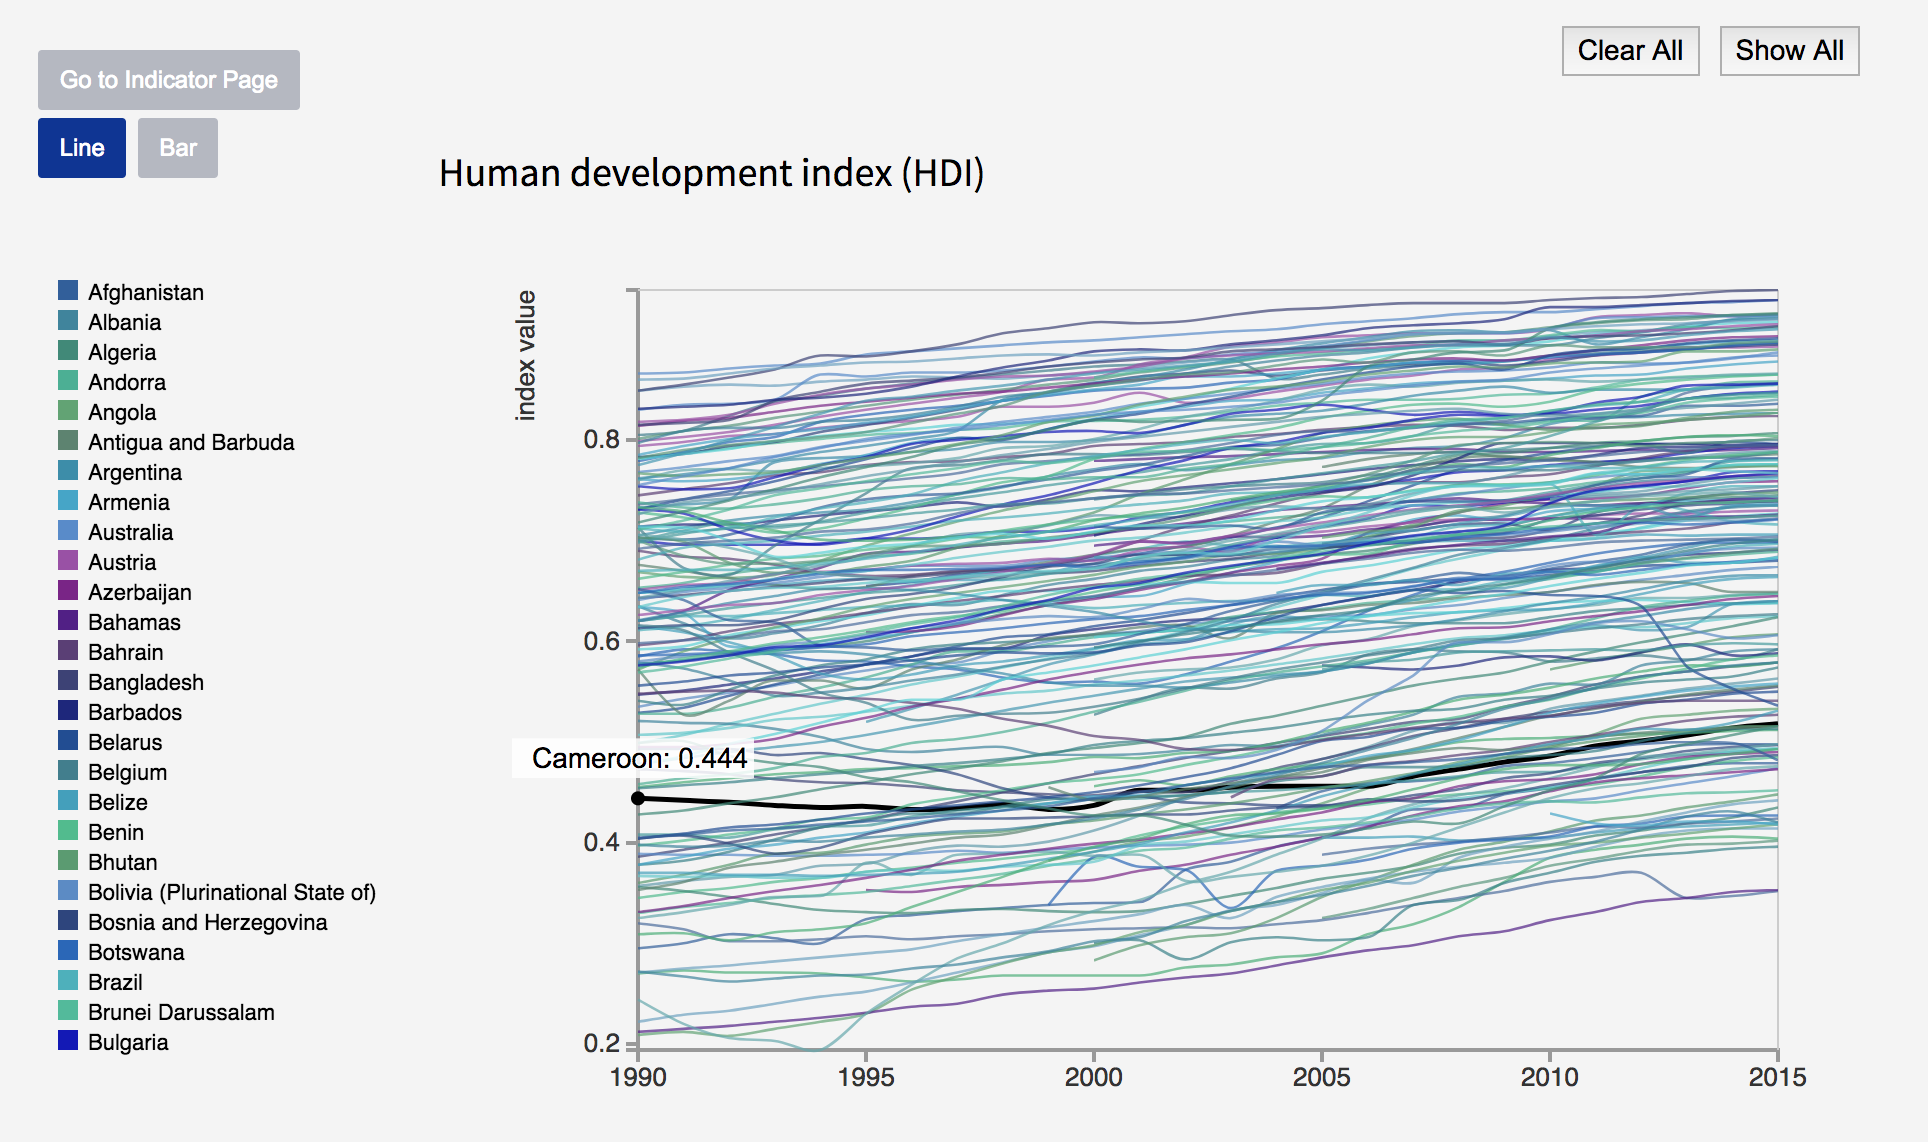
\includegraphics[width=0.4\textwidth]{undp}
    \caption{Line chart map from UNDP~\cite{UNDPlinechart}}
    \label{fig:undp}
\end{figure}
\begin{figure}[t]
    \centering
    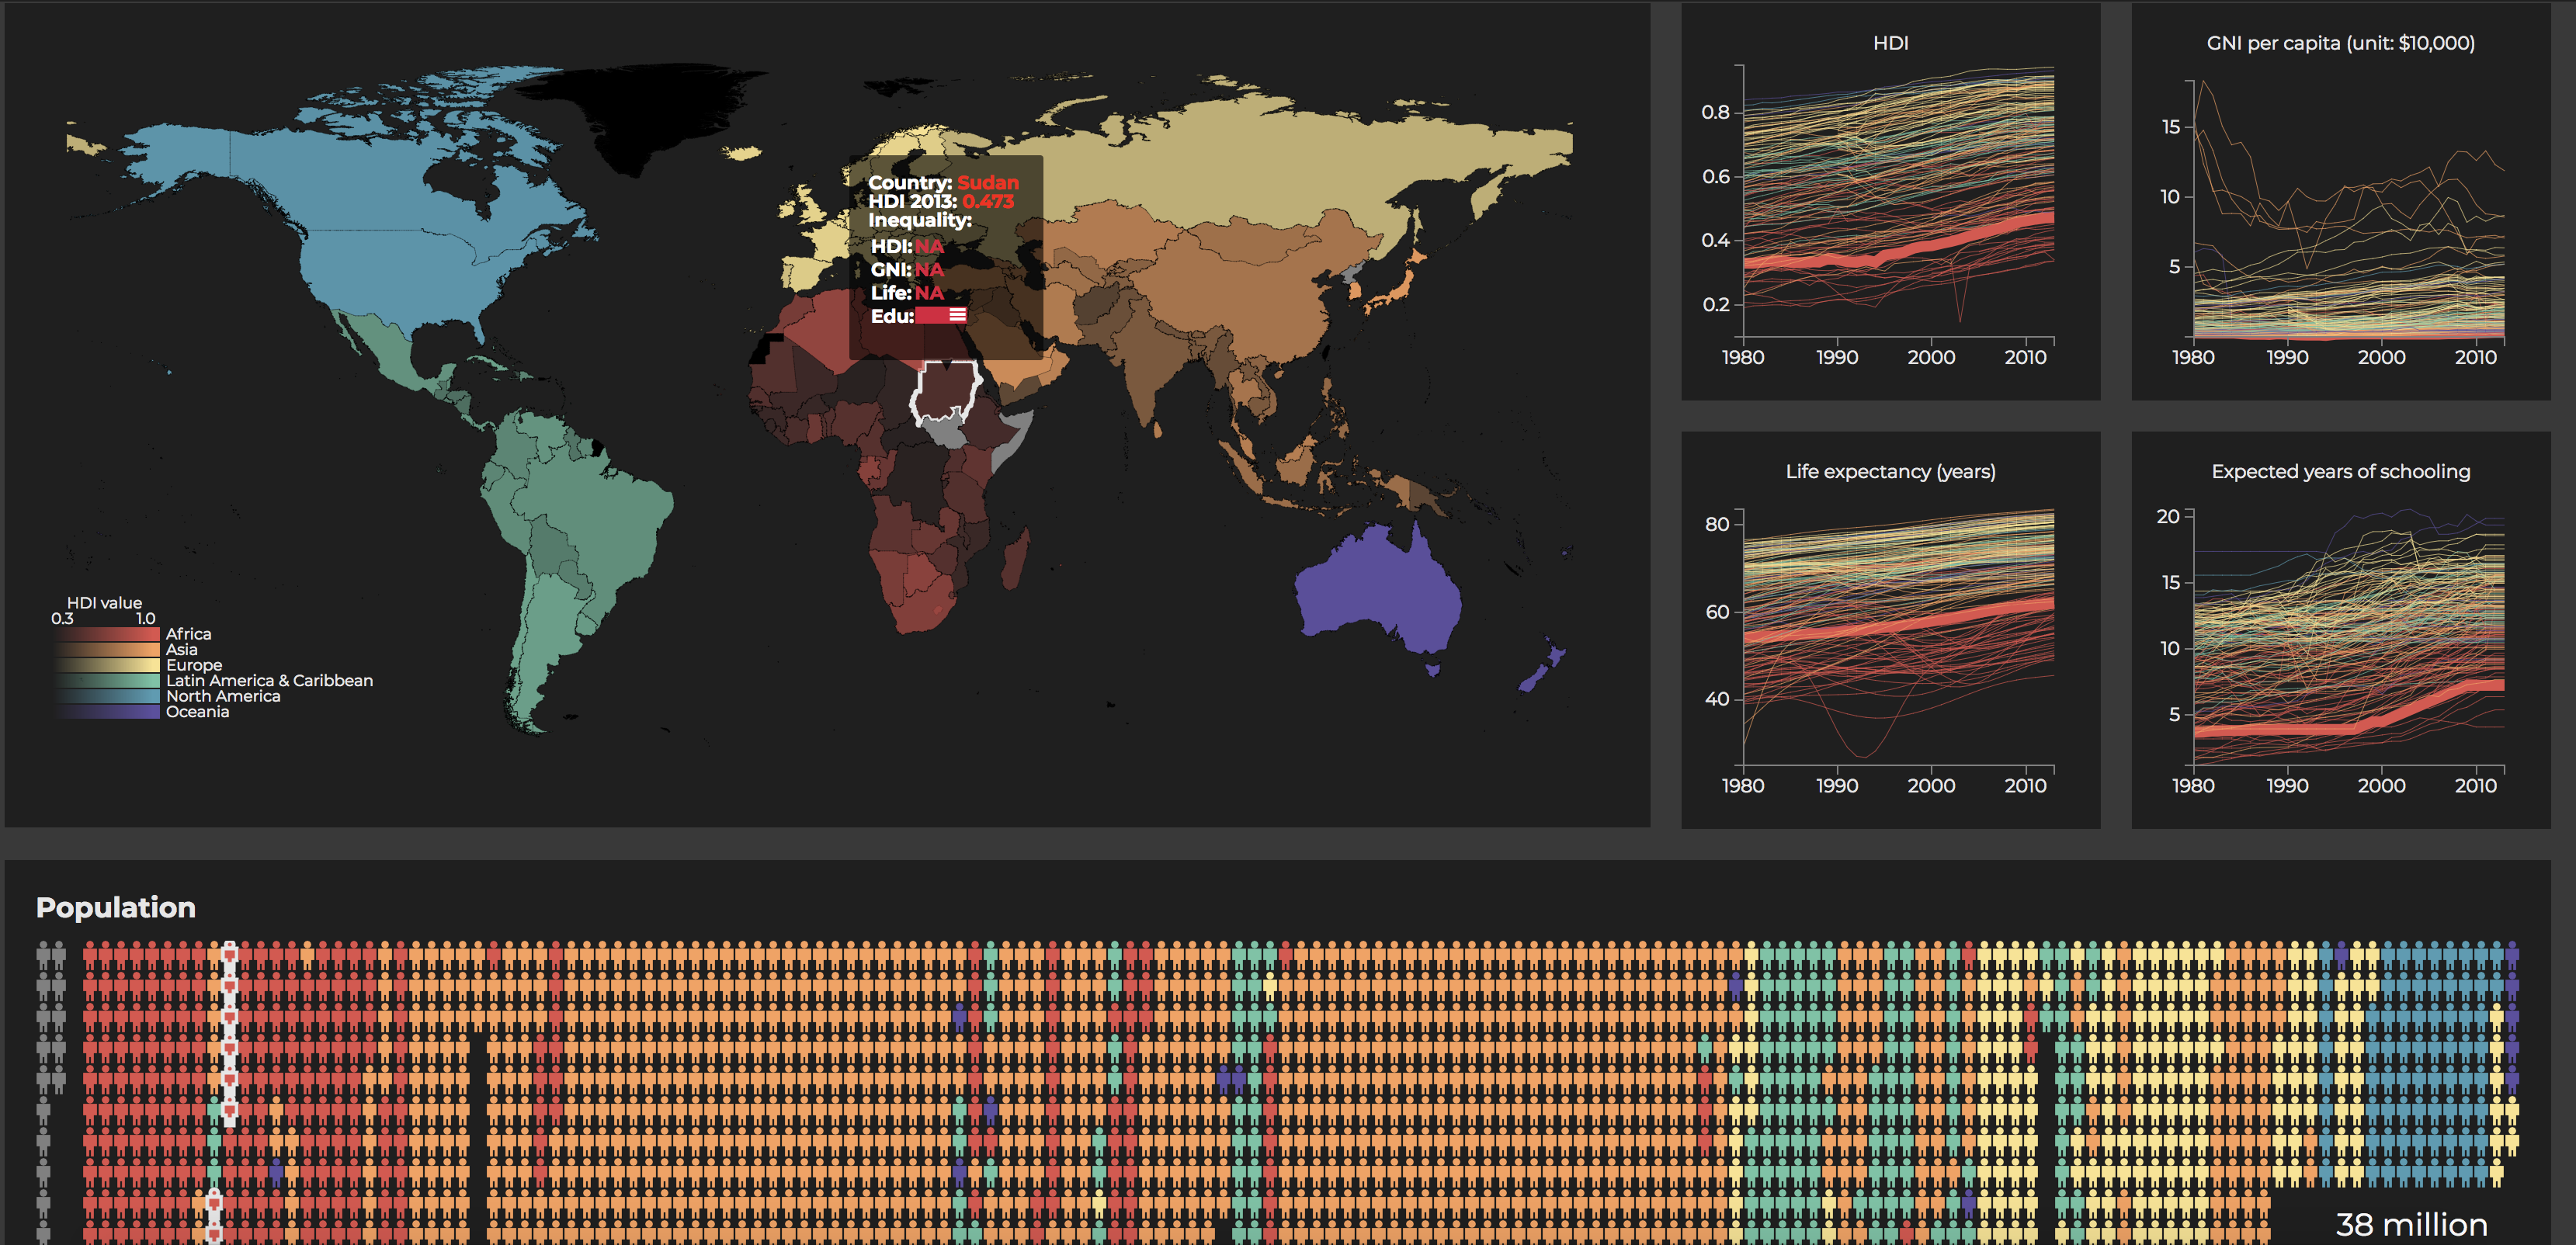
\includegraphics[width=0.4\textwidth]{amazon}
    \caption{Visualizing Human Development Index 2013~\cite{AmazonHDI}}
    \label{fig:amazon}
\end{figure}

\section{Data Source}
We use the HDI and its components data from the UNDP website~\cite{HDIcomponents,HDIinfo}, which can be downloaded into CSV files.

\section{Implementation}
We implement our tool in JavaScript because we want our tool to be a web-based application, which can be easy to access. JavaScript also has a library called D3.js that is used for producing data visualization in web browsers. Our tool can be run in web browsers. We use the built-in HTTP server , \texttt{SimpleHTTPServer}, to test and run our tool. Next we describe UI components and other tools we use in order to implement our web-based application.
\subsection{UI Components}
Our tool consists of multiple UI components as follows:
\begin{itemize}
	\item \textbf{World Map Layer}: we use the geojson data~\cite{geocountries}, which contains information for each country, such as country polygon coordinates to draw the world map and ISO ALPHA-3 code.
	\item \textbf{HDI Map layer}: HDI Map layer is built on top of World Map Layer, where we color each country polygon with a unique color based on how high its HDI is. As shown in Figure~\ref{fig:hdi}, the countries with high HDI value are colored bluish while the countries with low HDI value are colored reddish.
	\begin{figure}[t]
        \centering
		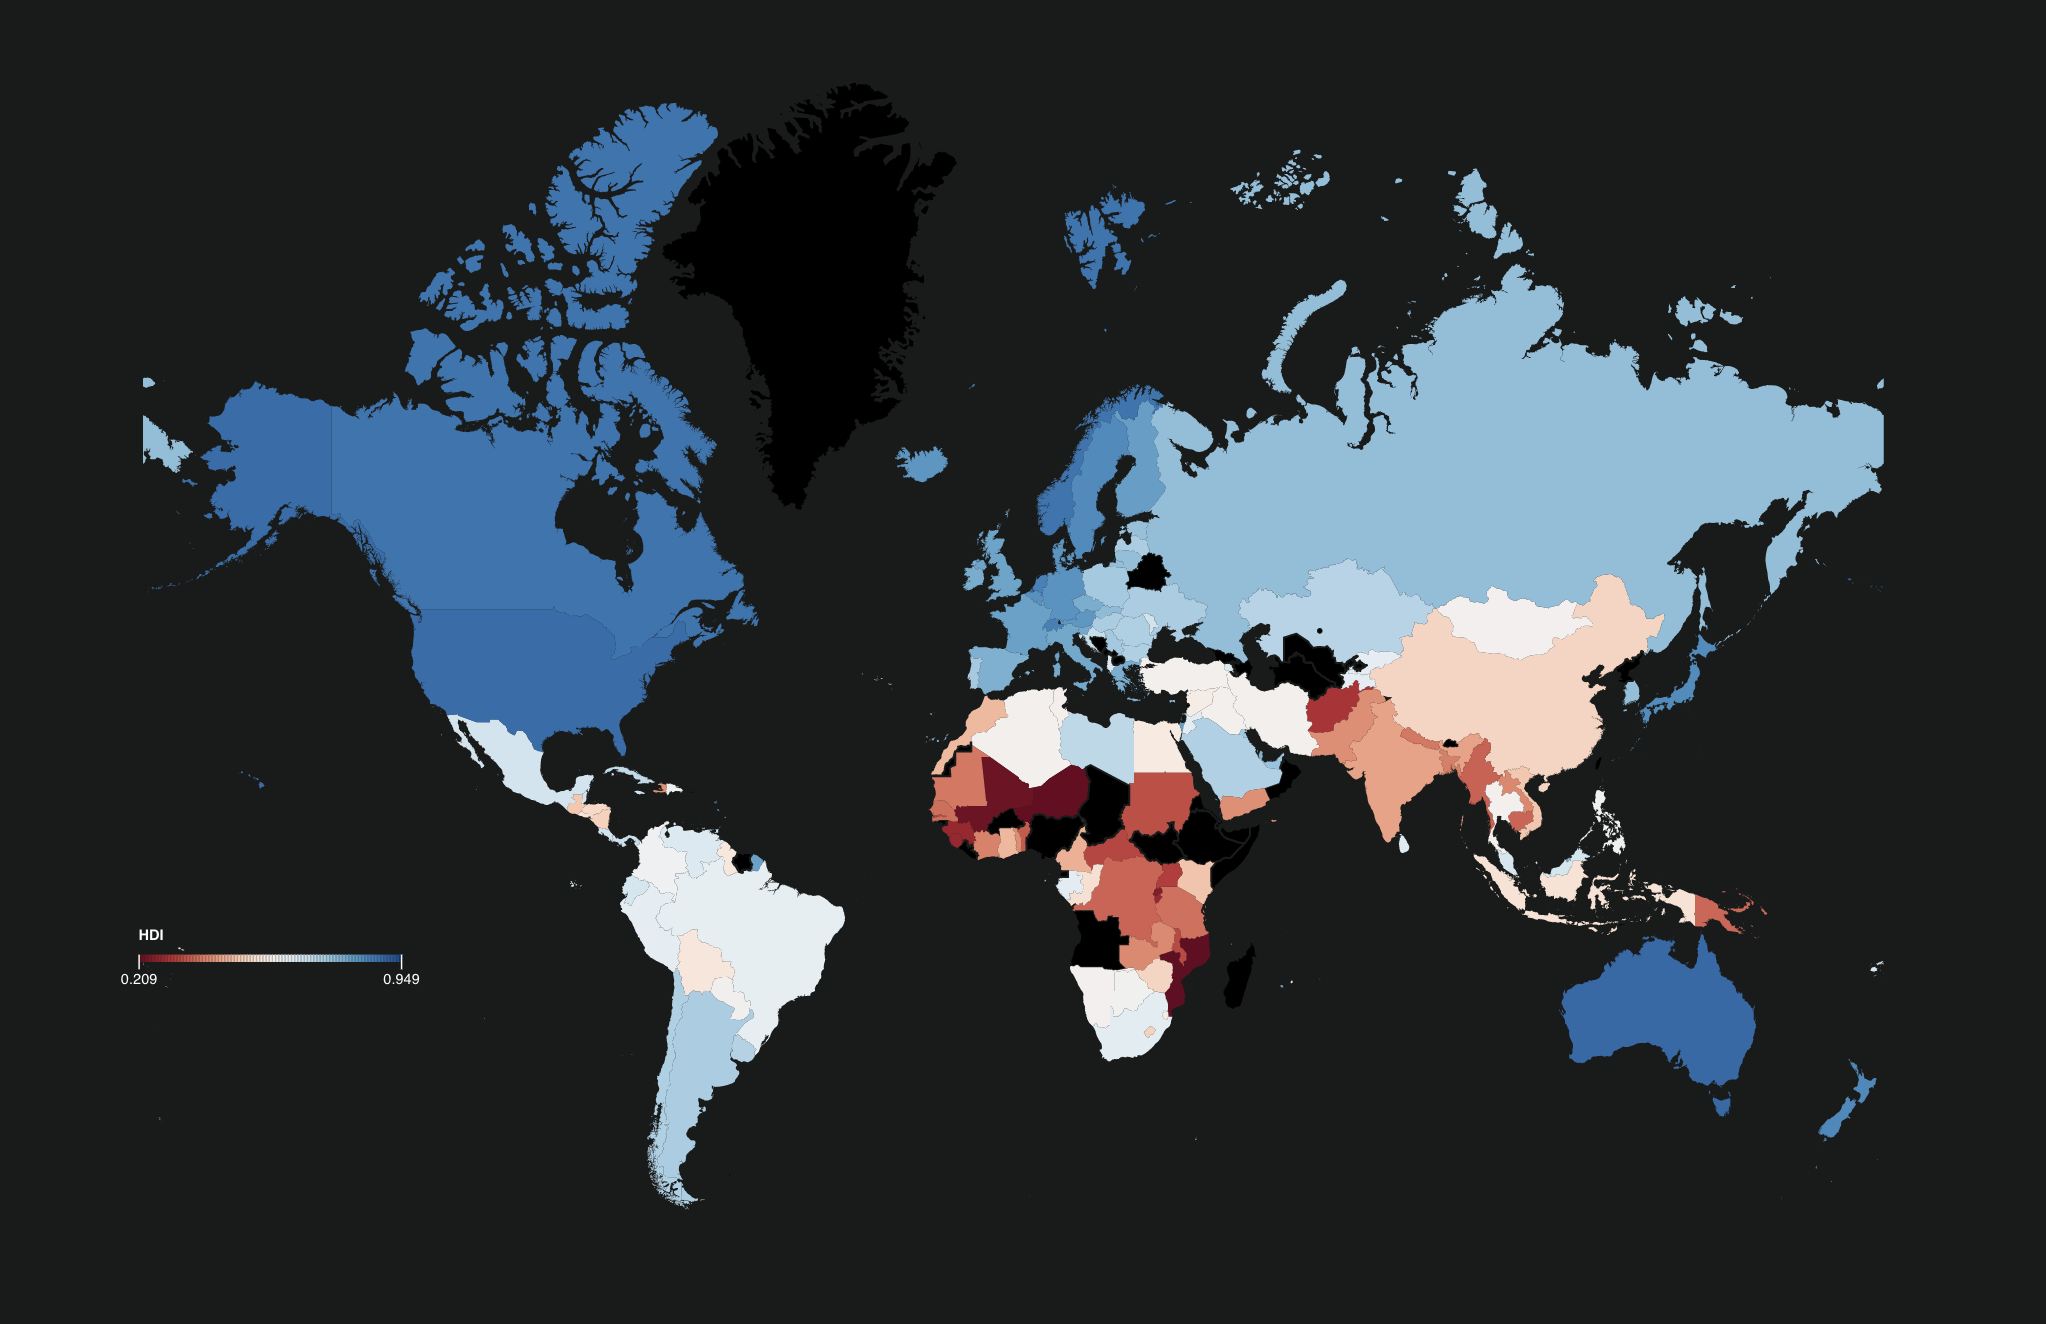
\includegraphics[width=0.4\textwidth]{hdiMap}
		\caption{HDI Map Layer}
		\label{fig:hdi}
	\end{figure}
	\item \textbf{Bivariate Map Layer}: Bivariate Map Layer shows a bivariate map. The legends of bivariate map have two axises. Each axis consists of three gradual colors, so there are nine combined colors in total. In our case, Bivariate Map Layer is used to compare two components of HDI and helps users any possible correlation between the two components. For example, Figure \ref{fig:bivariate} shows that most of the countries in the world have low values of GNI with high expected years of schooling.
	\begin{figure}[t]
        \centering
		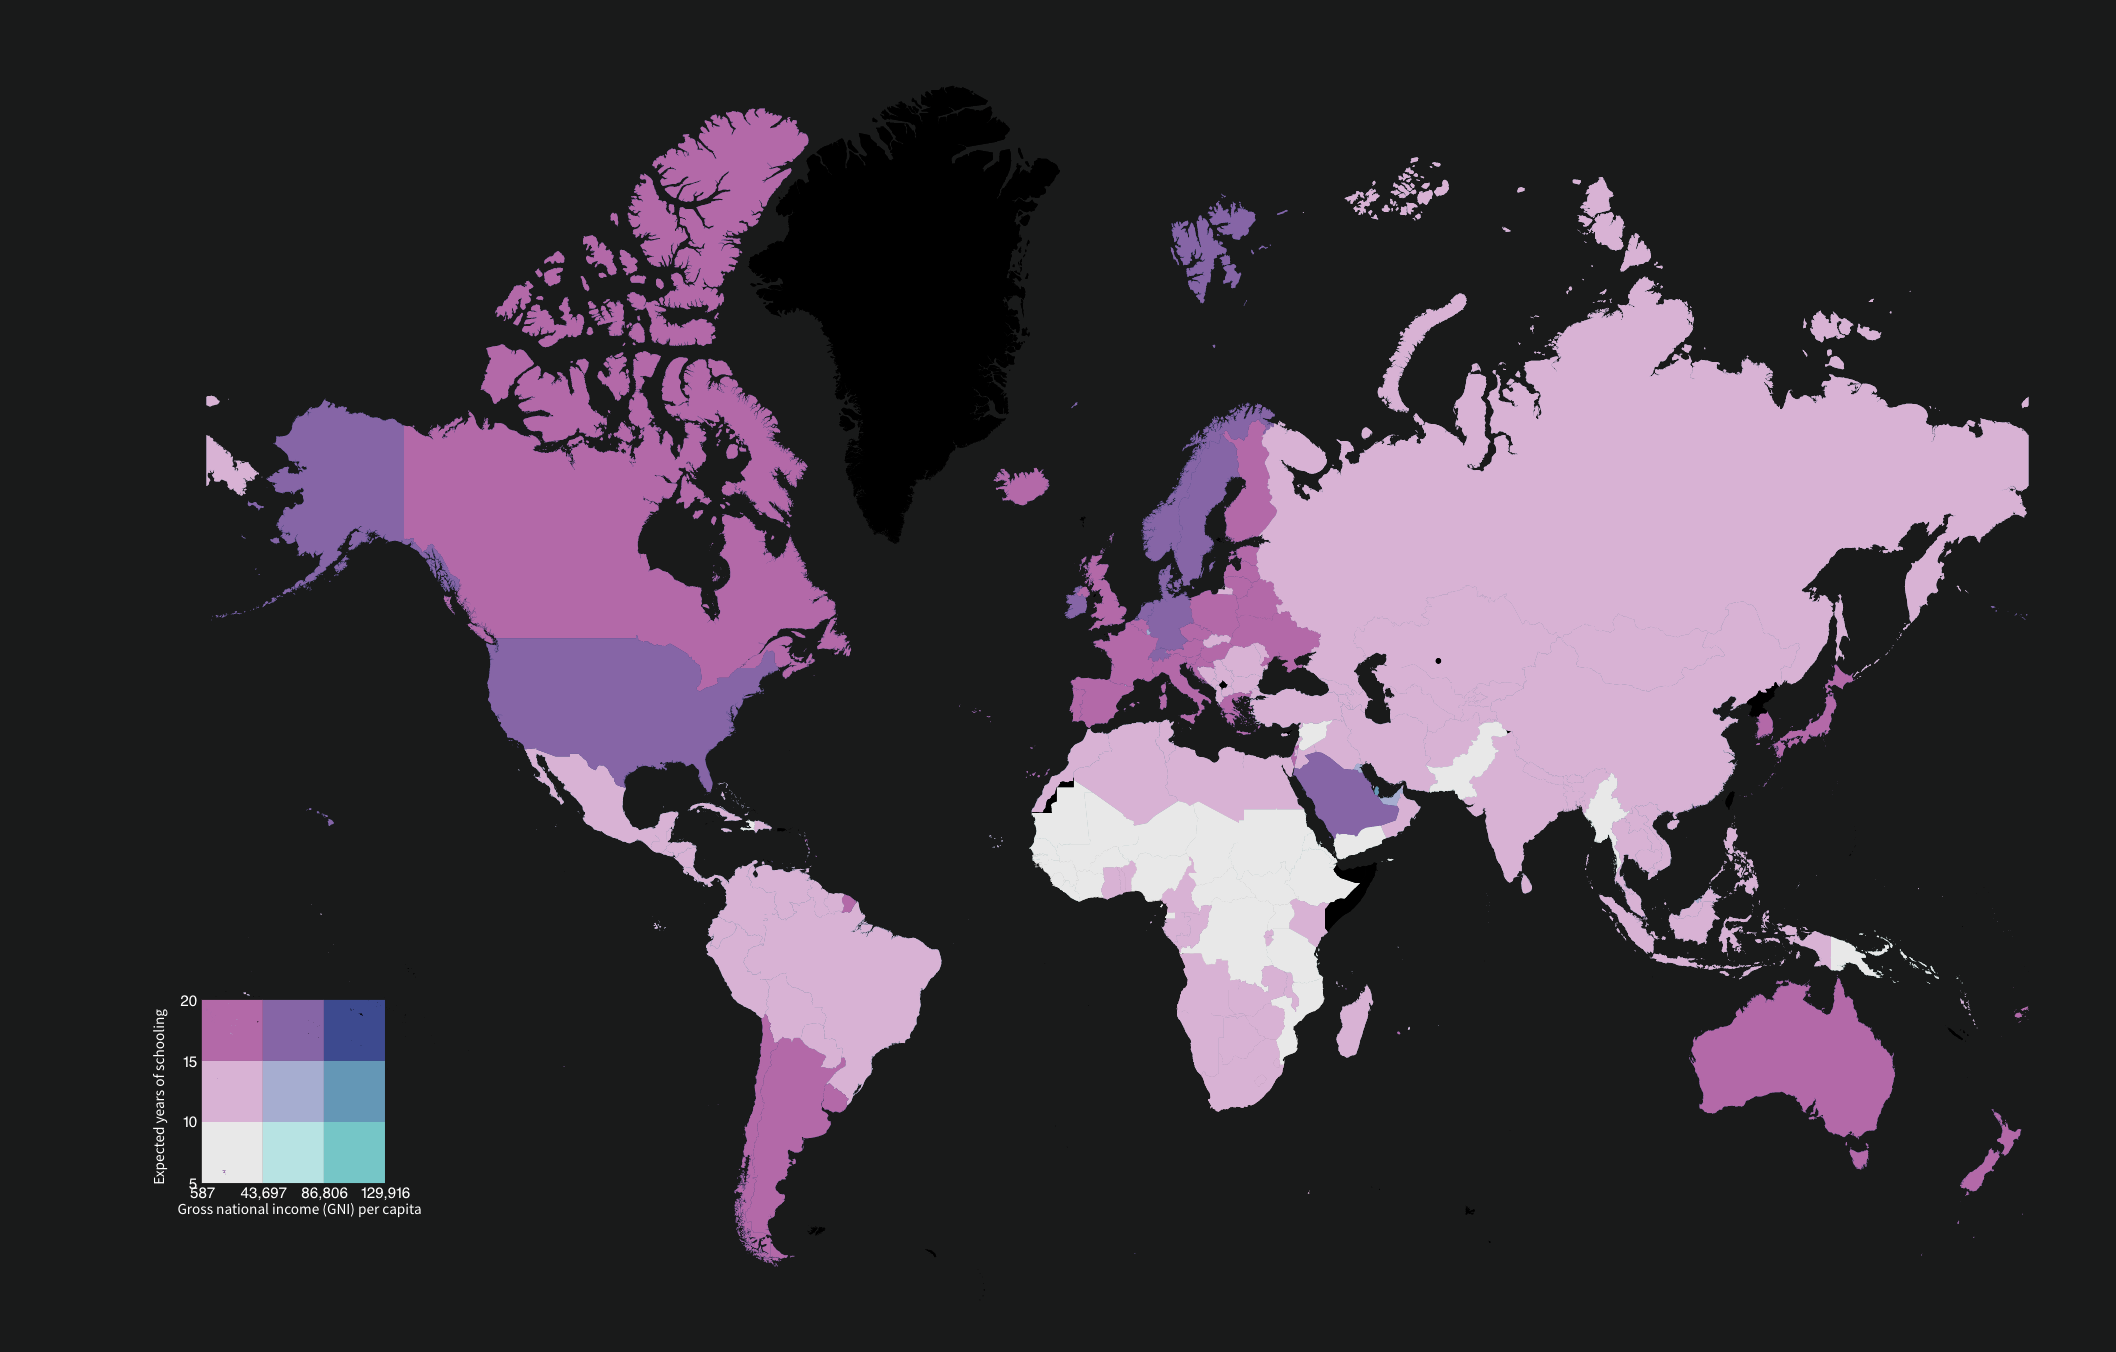
\includegraphics[width=0.4\textwidth]{bivariateMap}
		\caption{Bivaraite Map Layer}
		\label{fig:bivariate}
	\end{figure}
	\item \textbf{Parallel Coordinate Plot:} we use the parallel coordinate plot to show the values of HDI along with its components for all the countries. Each vertical axis represents a component. Thus, each line in the plot represents a country. We allow users to brush on each vertical axis to select a range of values they are interested in. For instance, if the users are only interested in data with high HDI value and low GNI value, they can simply brush on the vertical axises corresponding to those categories to filter out uninterested data (Figure~\ref{fig:parallel}).
	\begin{figure}[t]
        \centering
		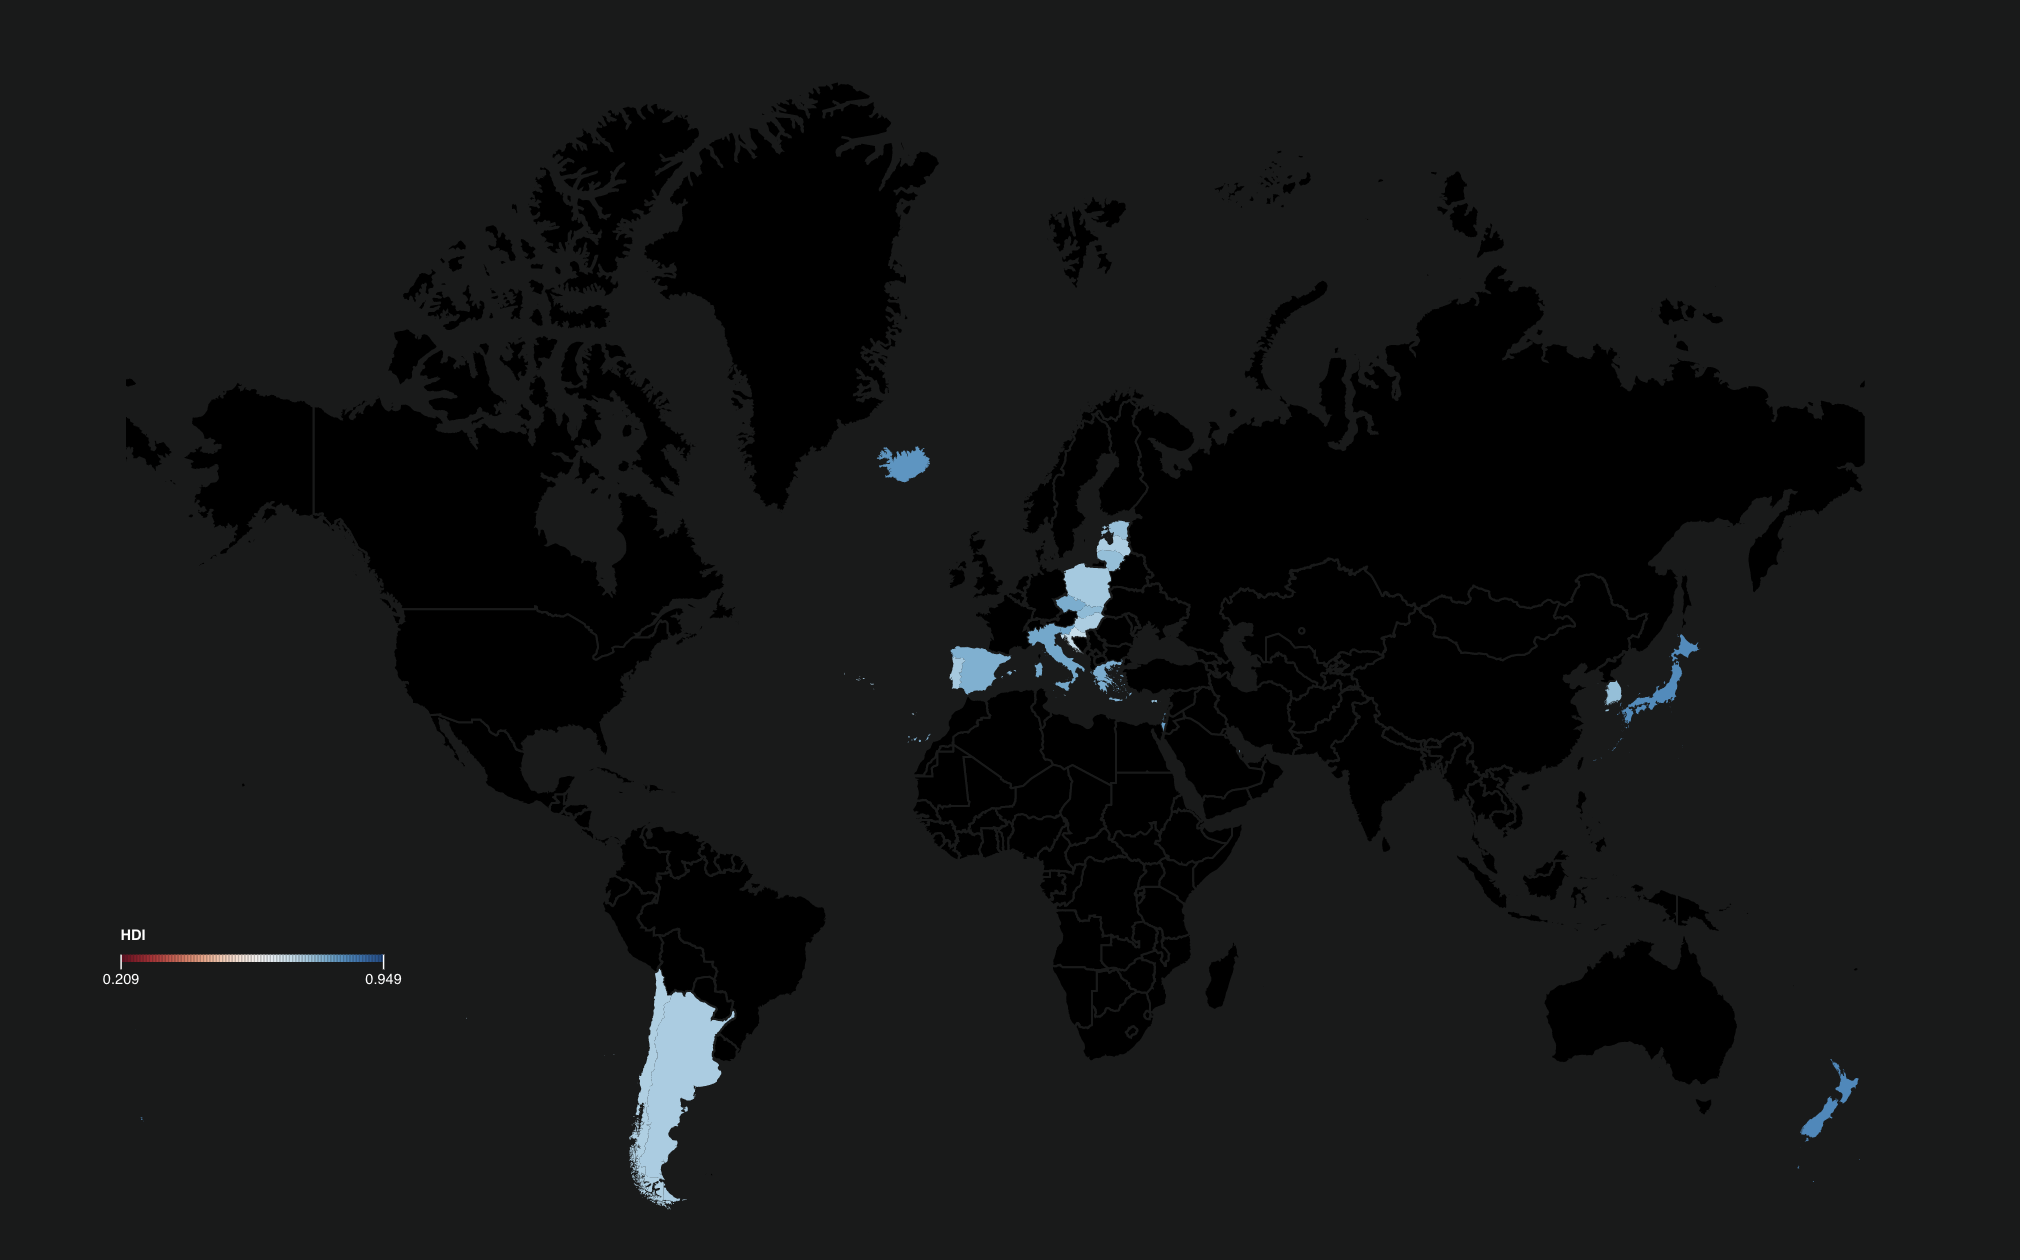
\includegraphics[width=0.4\textwidth]{filteredHdiMap}
		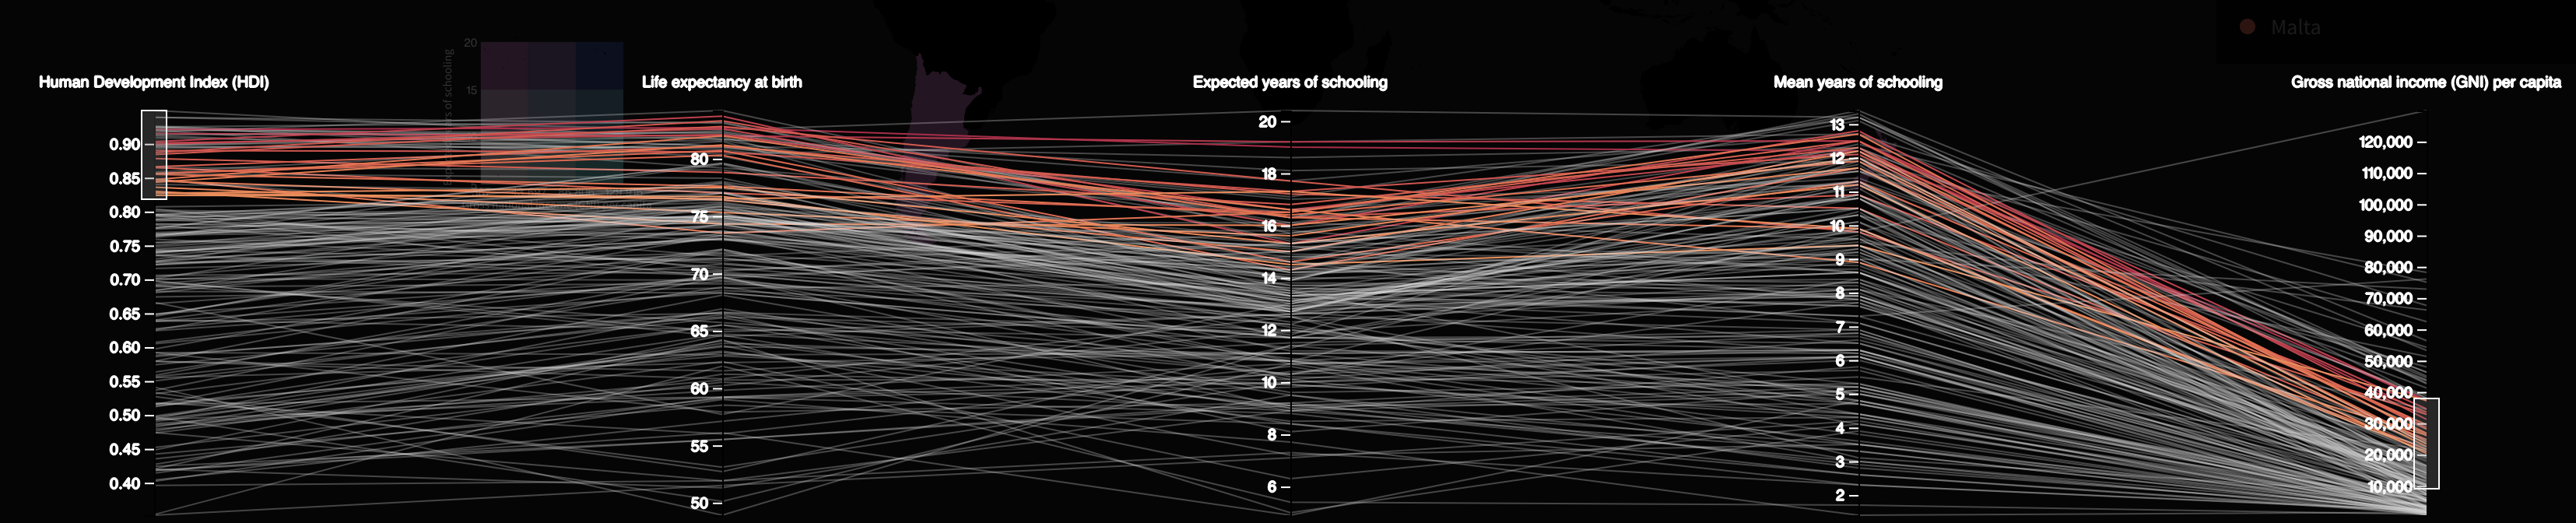
\includegraphics[width=0.4\textwidth]{parallelCoordGraph}
		\caption{Filter countries with high HDI and low GNI}
		\label{fig:parallel}
	\end{figure}
	\item \textbf{Controller:} there are three main components for the controller: map selector, year slider, and component selector. The map selector is responsible for selecting HDI Map Layer or Bivariate Map Layer to show. If HDI Map Layer is selected, the year slider will appear as well to allow users to slide between 1990 and 2015. Correspondingly, the HDI map will show the data from a specific year, which provides a historical view of the change in HDI over the years. If Bivariate Map Layer is selected, the year slider will be hidden and the component slider will be shown so that users can select which two components they are interested in (Figure~\ref{fig:controller}).
	\begin{figure}[t]
		\centering
        \subfloat[Select HDI map]{{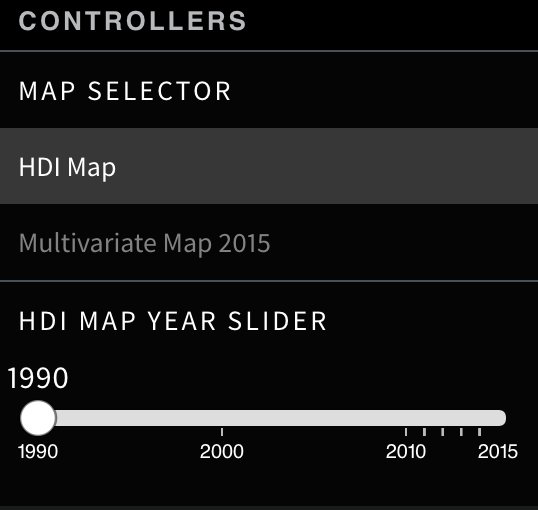
\includegraphics[width=3cm]{controllerHdi} }}%
        \qquad
        \subfloat[Select Bivariate Map]{{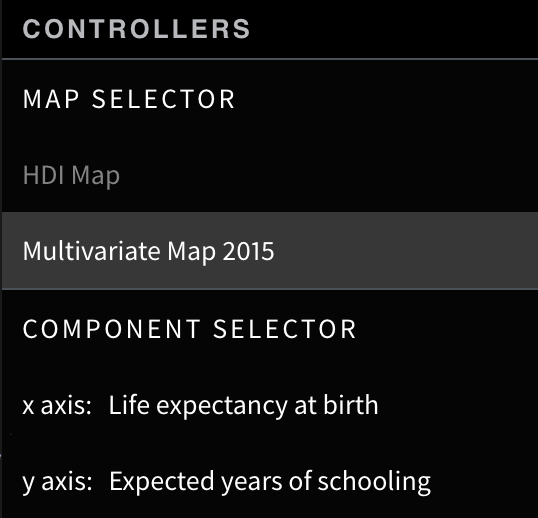
\includegraphics[width=3cm]{controllerBivariate} }}%
		\caption{Controller}
		\label{fig:controller}
	\end{figure}
    \item \textbf{Country Selector:} the country selector includes a search bar and a list of countries. The legend color next to each country name indicates the line color of the country shown in Parallel Coordinate Plot. The search bar allows users to select countries and helps user find a specific country on the world map. In additions, when users click on a country in the list, the corresponding country polygon on the world map and corresponding country line in the parallel coordinate plot will be highlighted. The detailed information of the country will be shown on the left side in Country Info Panel.
    \item \textbf{Country Info Panel:} the panel displays information about the country selected either from the map or from Country Selector. It contains two parts: statistics and a radar chart. \todo{add the figure and update ``xx'' $\rightarrow$} As shown in Figure xx, the radar chart provides a straightforward view of the percentiles of the HDI and its components of a selected country. It is easier for users to compare two countries from the radar chart than from simple texts, because the similarity of two countries can be captured by similar shapes (Figure~\ref{fig:panel}).
    \begin{figure}[t]
    	\centering
        \subfloat[New Zealand information]{{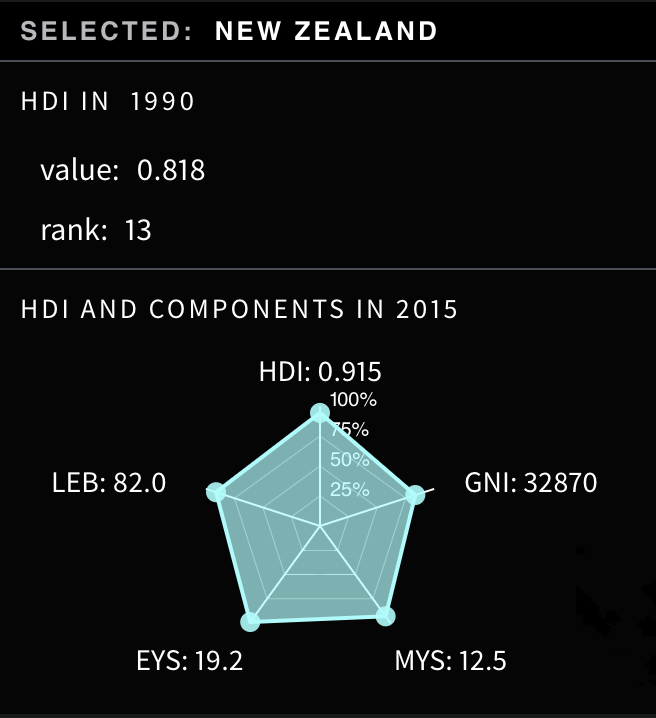
\includegraphics[width=3cm]{newZealand} }}%
        \qquad
        \subfloat[Korea information]{{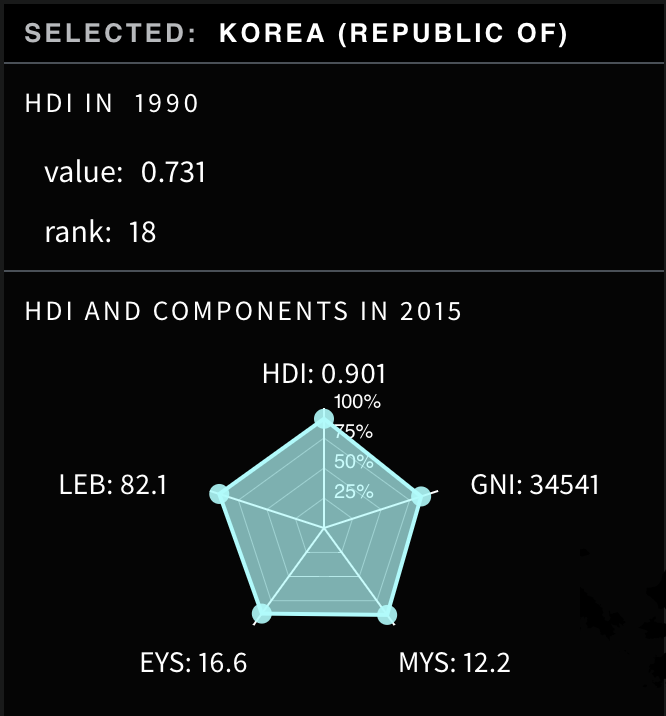
\includegraphics[width=3cm]{korea} }}%
    	\caption{New Zealand and Korea have close HDI ranks and values of HDI components}
    	\label{fig:panel}
    \end{figure}
\end{itemize}

\subsection{Design Logic}
To creating the preceding UI components, we have a main HTML file that includes one HTML \texttt{<div>} wrapper with a unique id for each UI component. Each UI component is implemented in a single JS file as module, where we extract the corresponding wrapper div from the main HTML file to build visualizations. For the charts and map, we use D3.js to create svg and inner layers. For communication between different UI components, we use d3.dispatch to generate event dispatchers and event listeners.  We also have a global JS file to shares global variables among all the components. As for styling, we create one CSS file for each component to independently set styles of components.

\section{Visualization Result and Conclusion}
Our visualization tool allows users to see the relationship between HDI and its components. As we can see from Figure~\ref{fig:parallelplot}, almost all the countries with high HDI have relatively high values of the four components (LEB, EYS, MYS, GNI). In additions, the bivariate map (Figure~\ref{fig:bivariate}) shows an interesting finding: most of the countries have close values of GNI per capita, regardless of how many expected years of schooling people have. Figure~\ref{fig:parallelplot} shows that all the countries except only one country have GNI per capita under 80000 in 2015. The only one country with the highest GNI per capita is Qatar. Another finding is that the countries located in the lower part of the earth tend to have low expected years of schooling as shown in our tool by showing only countries (on the world map) with values of the low expected years of schooling. The world map (Figure~\ref{fig:hdi}) also leads to the conclusion that Africa is the continent that has the relatively low human development as most of the countries in Africa have low HDI. However, by using the year slider controller, we can see that the majority of the countries have been developed in the past several years, because their HDI values are increasing as the years go by. 

\begin{figure}[t]
    \centering
    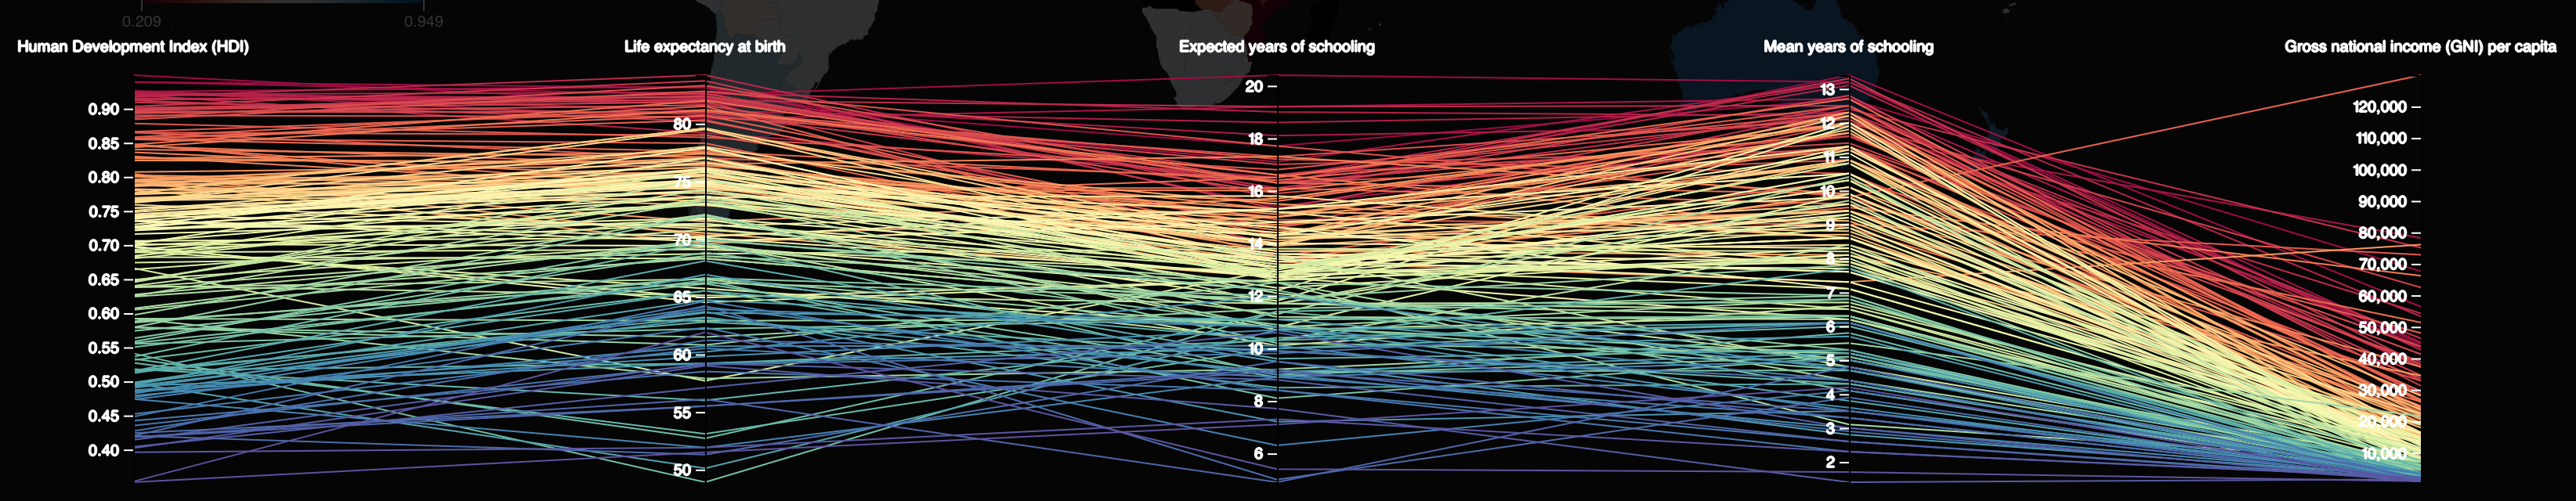
\includegraphics[width=0.4\textwidth]{parallelplot}
    \caption{Parallel Coordinate Plot showing the HDI and its components of each country in 2015}
    \label{fig:parallelplot}
\end{figure}

\section{Conclusion}




\bibliographystyle{abbrv-doi}
\bibliography{main}
\end{document}
